% !TeX root = Sprawozdanie.tex

\documentclass[12pt, a4paper]{article}
\usepackage{graphicx}
\usepackage[T1]{fontenc}
\usepackage[margin=0.75in,footskip=0.25in]{geometry}
\usepackage[polish]{babel}
\graphicspath{{./plots/}}

\title{Metody numeryczne - Badanie wskaźnika giełdowego MACD}
\author{Krzysztof Nasuta, s193328}
\date{\today}

\begin{document}
\maketitle

\section{Wstęp}
Celem projektu jest zaimplementowanie wskaźnika giełdowego MACD (ang. Moving Average Convergence Divergence)
oraz przeprowadzenie analizy jego skuteczności. Celem wskaźnika MACD jest wykrywanie oraz rozpoznawanie
zmian trendów na rynku finansowym. MACD składa się z 2 szeregów czasowych: linii MACD oraz linii sygnałowej.
Linia MACD uzyskiwana jest jako różnica pomiędzy 2 średnimi: długoterminową oraz krótkoterminową.
Linia sygnałowa wyliczana jest jako średnia z powstałej linii MACD. Do wyliczenia średnich często
używana jest wykładnicza średnia krocząca (ang. exponential moving average, EMA). W projekcie linię MACD uzyskano jako różnicę
pomiędzy 12-dniową wykładniczą średnią kroczącą oraz 26-dniową wykładniczą średnią kroczącą. Linia sygnałowa to 
9-dniowa wykładnicza średnia krocząca z linii MACD.


\begin{figure}[h]
    \centering
    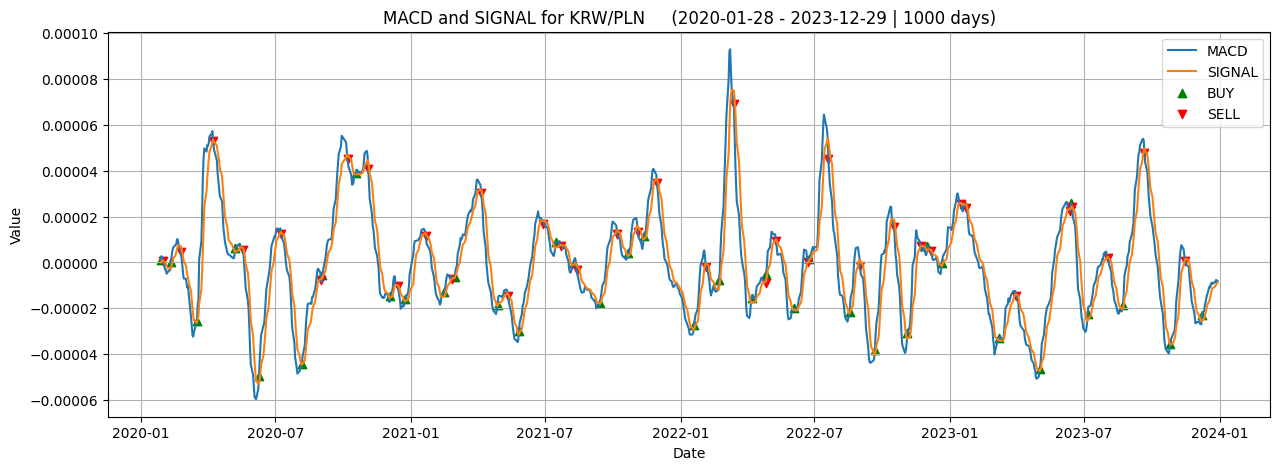
\includegraphics[width=1.0\textwidth]{krw_pln_macd_signal.png}
    \caption{Wykres kursu walutowego KRW/PLN oraz wskaźników MACD oraz sygnałowego.}
    \label{fig:krw_pln_macd_signal}
\end{figure}

\end{document}